
%(BEGIN_QUESTION)
% Copyright 2006, Tony R. Kuphaldt, released under the Creative Commons Attribution License (v 1.0)
% This means you may do almost anything with this work of mine, so long as you give me proper credit

A water storage vessel is elevated by a tower structure, to provide a natural source of water pressure to all points of use below:

$$\includegraphics[width=15.5cm]{i00253x01.eps}$$

A pressure-sensing level transmitter is presently located at the base of the vessel, at the top of the tower structure, to measure water level inside the vessel.  It has a calibrated range of 0 to 10 feet (0 to 120 inches W.C.).  Unfortunately, the water inside the transmitter sometimes freezes in the winter months, preventing operation of the level measurement system.  The water inside the storage vessel and the large pipes never freezes, because there is enough circulation as a result of water usage to raise the temperature and prevent ice crystals from forming.

It is decided to move the transmitter to ground level, at the base of the tower, so that it may be located inside a small, heated shelter where it will never freeze.  By connecting the transmitter directly to the large water pipe carrying water from the vessel to the points of use, the hydrostatic pressure will still be measurable at this point:

$$\includegraphics[width=15.5cm]{i00253x02.eps}$$

Calculate the new calibration points (lower and upper range-values) for the transmitter in its new location.  Also calculate the water level in the vessel when the transmitter output is 13.7 mA, and the amount of hydrostatic pressure at that point in units of PSI.

\vskip 10pt

Finally, identify whether the transmitter move resulted in a shift of its {\it zero}, a shift in its {\it span}, or both.

\underbar{file i00253}
%(END_QUESTION)





%(BEGIN_ANSWER)

Lower range-values: 100 feet W.C. input (1200 inches W.C.) = 4 mA output

Upper range-values: 110 feet W.C. input (1320 inches W.C.) = 20 mA output

\vskip 10pt

Water level in vessel at 13.7 mA = 6.0625 feet ; applied pressure = 45.98 PSI

%(END_ANSWER)





%(BEGIN_NOTES)

Moving the transmitter to the bottom of the tower introduced a large {\it zero} shift into its calibrated range, but there was no effect on span.

\vskip 10pt

I once moved a water level transmitter in this very manner: from the top of the tower to ground level, and for the same reason.  One issue I faced was being able to find a transmitter that could handle such a large amount of zero suppression with such a relatively small span.  The ultimate factor in deciding the correct transmitter model was adequate {\it rangedown}: being able to turn down the span to such a small amount while maintaining a large zero shift.

The original transmitter was a Rosemount 1151.  I was unable to turn down the span on this transmitter far enough, and ended up having to replace it with a (newer) Rosemount model 3051 which was a relatively new product at that time (mid 1990's).

%INDEX% Measurement, level: hydrostatic pressure
%INDEX% Process: water storage tank (elevated)

%(END_NOTES)


